% Options for packages loaded elsewhere
\PassOptionsToPackage{unicode}{hyperref}
\PassOptionsToPackage{hyphens}{url}
%
\documentclass[
]{article}
\usepackage{amsmath,amssymb}
\usepackage{lmodern}
\usepackage{iftex}
\ifPDFTeX
  \usepackage[T1]{fontenc}
  \usepackage[utf8]{inputenc}
  \usepackage{textcomp} % provide euro and other symbols
\else % if luatex or xetex
  \usepackage{unicode-math}
  \defaultfontfeatures{Scale=MatchLowercase}
  \defaultfontfeatures[\rmfamily]{Ligatures=TeX,Scale=1}
\fi
% Use upquote if available, for straight quotes in verbatim environments
\IfFileExists{upquote.sty}{\usepackage{upquote}}{}
\IfFileExists{microtype.sty}{% use microtype if available
  \usepackage[]{microtype}
  \UseMicrotypeSet[protrusion]{basicmath} % disable protrusion for tt fonts
}{}
\makeatletter
\@ifundefined{KOMAClassName}{% if non-KOMA class
  \IfFileExists{parskip.sty}{%
    \usepackage{parskip}
  }{% else
    \setlength{\parindent}{0pt}
    \setlength{\parskip}{6pt plus 2pt minus 1pt}}
}{% if KOMA class
  \KOMAoptions{parskip=half}}
\makeatother
\usepackage{xcolor}
\usepackage[margin=1in]{geometry}
\usepackage{color}
\usepackage{fancyvrb}
\newcommand{\VerbBar}{|}
\newcommand{\VERB}{\Verb[commandchars=\\\{\}]}
\DefineVerbatimEnvironment{Highlighting}{Verbatim}{commandchars=\\\{\}}
% Add ',fontsize=\small' for more characters per line
\usepackage{framed}
\definecolor{shadecolor}{RGB}{248,248,248}
\newenvironment{Shaded}{\begin{snugshade}}{\end{snugshade}}
\newcommand{\AlertTok}[1]{\textcolor[rgb]{0.94,0.16,0.16}{#1}}
\newcommand{\AnnotationTok}[1]{\textcolor[rgb]{0.56,0.35,0.01}{\textbf{\textit{#1}}}}
\newcommand{\AttributeTok}[1]{\textcolor[rgb]{0.77,0.63,0.00}{#1}}
\newcommand{\BaseNTok}[1]{\textcolor[rgb]{0.00,0.00,0.81}{#1}}
\newcommand{\BuiltInTok}[1]{#1}
\newcommand{\CharTok}[1]{\textcolor[rgb]{0.31,0.60,0.02}{#1}}
\newcommand{\CommentTok}[1]{\textcolor[rgb]{0.56,0.35,0.01}{\textit{#1}}}
\newcommand{\CommentVarTok}[1]{\textcolor[rgb]{0.56,0.35,0.01}{\textbf{\textit{#1}}}}
\newcommand{\ConstantTok}[1]{\textcolor[rgb]{0.00,0.00,0.00}{#1}}
\newcommand{\ControlFlowTok}[1]{\textcolor[rgb]{0.13,0.29,0.53}{\textbf{#1}}}
\newcommand{\DataTypeTok}[1]{\textcolor[rgb]{0.13,0.29,0.53}{#1}}
\newcommand{\DecValTok}[1]{\textcolor[rgb]{0.00,0.00,0.81}{#1}}
\newcommand{\DocumentationTok}[1]{\textcolor[rgb]{0.56,0.35,0.01}{\textbf{\textit{#1}}}}
\newcommand{\ErrorTok}[1]{\textcolor[rgb]{0.64,0.00,0.00}{\textbf{#1}}}
\newcommand{\ExtensionTok}[1]{#1}
\newcommand{\FloatTok}[1]{\textcolor[rgb]{0.00,0.00,0.81}{#1}}
\newcommand{\FunctionTok}[1]{\textcolor[rgb]{0.00,0.00,0.00}{#1}}
\newcommand{\ImportTok}[1]{#1}
\newcommand{\InformationTok}[1]{\textcolor[rgb]{0.56,0.35,0.01}{\textbf{\textit{#1}}}}
\newcommand{\KeywordTok}[1]{\textcolor[rgb]{0.13,0.29,0.53}{\textbf{#1}}}
\newcommand{\NormalTok}[1]{#1}
\newcommand{\OperatorTok}[1]{\textcolor[rgb]{0.81,0.36,0.00}{\textbf{#1}}}
\newcommand{\OtherTok}[1]{\textcolor[rgb]{0.56,0.35,0.01}{#1}}
\newcommand{\PreprocessorTok}[1]{\textcolor[rgb]{0.56,0.35,0.01}{\textit{#1}}}
\newcommand{\RegionMarkerTok}[1]{#1}
\newcommand{\SpecialCharTok}[1]{\textcolor[rgb]{0.00,0.00,0.00}{#1}}
\newcommand{\SpecialStringTok}[1]{\textcolor[rgb]{0.31,0.60,0.02}{#1}}
\newcommand{\StringTok}[1]{\textcolor[rgb]{0.31,0.60,0.02}{#1}}
\newcommand{\VariableTok}[1]{\textcolor[rgb]{0.00,0.00,0.00}{#1}}
\newcommand{\VerbatimStringTok}[1]{\textcolor[rgb]{0.31,0.60,0.02}{#1}}
\newcommand{\WarningTok}[1]{\textcolor[rgb]{0.56,0.35,0.01}{\textbf{\textit{#1}}}}
\usepackage{graphicx}
\makeatletter
\def\maxwidth{\ifdim\Gin@nat@width>\linewidth\linewidth\else\Gin@nat@width\fi}
\def\maxheight{\ifdim\Gin@nat@height>\textheight\textheight\else\Gin@nat@height\fi}
\makeatother
% Scale images if necessary, so that they will not overflow the page
% margins by default, and it is still possible to overwrite the defaults
% using explicit options in \includegraphics[width, height, ...]{}
\setkeys{Gin}{width=\maxwidth,height=\maxheight,keepaspectratio}
% Set default figure placement to htbp
\makeatletter
\def\fps@figure{htbp}
\makeatother
\setlength{\emergencystretch}{3em} % prevent overfull lines
\providecommand{\tightlist}{%
  \setlength{\itemsep}{0pt}\setlength{\parskip}{0pt}}
\setcounter{secnumdepth}{-\maxdimen} % remove section numbering
\ifLuaTeX
  \usepackage{selnolig}  % disable illegal ligatures
\fi
\IfFileExists{bookmark.sty}{\usepackage{bookmark}}{\usepackage{hyperref}}
\IfFileExists{xurl.sty}{\usepackage{xurl}}{} % add URL line breaks if available
\urlstyle{same} % disable monospaced font for URLs
\hypersetup{
  pdftitle={Introduction à R},
  pdfauthor={ibrahima SAGNO},
  hidelinks,
  pdfcreator={LaTeX via pandoc}}

\title{Introduction à R}
\author{ibrahima SAGNO}
\date{2023-06-26}

\begin{document}
\maketitle

\hypertarget{quest---ce-que-r}{%
\subsection{Qu'est - ce que R ?}\label{quest---ce-que-r}}

Développé par \textbf{Ross Lhaka} et \textbf{Robert Gentleman} à
l'université d'Auckland, en Nouvelle-Zélande dans les années 1990, R est
d'abord un langage de programmation et un environnement logiciel ``Open
source''. Il a été conçu pour l'\textbf{analyse statistique , la
manipulation des données et la visualisation}. L'appelation
\textbf{``Open source''} désigne un logiciel ou un programme dont la
conception,le code source et les droits de distribution sont ouverts et
accessibles à tous.

A cet effet, R dispose d'une grande communauté d'utilisateurs. EN
naviguant sur le web , vous trouverez des forums, des listes de
diffusion, ou encore des groupes dédiées à R dans lesquels vous
trouverez réponse à la plupart de vos inquiétudes.

De plus, R est largement utilisé dans le monde universitaire et dans le
monde de la recherche là où on fait beaucoup appel à des préceptes
statistiques.

\hypertarget{pourquoi-r}{%
\subsection{Pourquoi R ?}\label{pourquoi-r}}

Il existe pluisieurs langages de programmation des plus simples au plus
complexe. Pourquoi alors le choix d'écrire un livre sur R ? Il y'a des
années maintenant que j'ai pour ambition d'initier un public non initié
aux concetps de l'Analytics. Cependant, R est le langage qui se
rapproche le plus des fomules \textbf{Excel} que nous utilisons depuis
le collège. C'est pour cette raison pédagogique et linéaire que mon
choix porte sur R d'autant plus que c'est le prmier langage que j'ai
appris durant mes années de licence.

\hypertarget{que-contient-ce-livre}{%
\subsection{Que contient ce livre ?}\label{que-contient-ce-livre}}

Ce livre a l'avantage d'être concis et à la fois. Il comprendra 7
chapitres allant de l'installation de R Studio, aux utilisations
avancées de R à savoir la création des fonctions, l'utlisation des
boucles en passant par l'analyse statistique et la visualisation des
données.

Comme je le disais en Introduction, R est un logiciel open source.
Durant le déroulé de ce livre, nous utiliserons principalement des
``Packages'' , c'est à dire des bibliothèques conçues par la communauté
et regroupant plusieurs fonctionnalités.

\hypertarget{chapitre-1-installation-et-configuration-de-r}{%
\subsection{Chapitre 1: Installation et Configuration de
R}\label{chapitre-1-installation-et-configuration-de-r}}

Vous pouvez installer \textbf{R} sur les principales distributions à
savoir Windows, macOS, et Linux.

\hypertarget{tuxe9luxe9chargement-de-r}{%
\subsubsection{Téléchargement de R:}\label{tuxe9luxe9chargement-de-r}}

Pour télécharger le programme d'installation de R, rendez-vous sur le
site officiel du \href{https://www.r-project.org/}{projet R}.\\
- Cliquez sur le lien de téléchargement correspondant à votre système
d'exploitation (Windows, macOS, Linux).\\
- Choisissez un miroir de téléchargement proche de votre emplacement
géographique en cliquant sur le lien
\href{https://cran.r-project.org/mirrors.html}{CRAN}. Le lien vers la
France est disponible \href{https://pbil.univ-lyon1.fr/CRAN/}{ici}.\\
- Téléchargez le fichier d'installation de R correspondant à votre
système d'exploitation.

\hypertarget{installation-de-r}{%
\subsubsection{Installation de R}\label{installation-de-r}}

\begin{itemize}
\tightlist
\item
  Exécuter le fichier d'installation téléchargé\\
\item
  Suivez les instructions de l'assisstant d'installation pour configurer
  R sur votre système d'exploitation.\\
\item
  Choississez votre repertoire d'installation et les options de
  configuration selon vos préférences.
\end{itemize}

\hypertarget{configuration-de-lenvironnement-de-duxe9veloppement-intuxe9gruxe9-ide-studio}{%
\subsubsection{Configuration de l'environnement de développement intégré
(IDE
Studio)}\label{configuration-de-lenvironnement-de-duxe9veloppement-intuxe9gruxe9-ide-studio}}

un IDE fourni un ensemble d'outils , d'éditeurs de code, de débogueurs ,
de consoles et d'autres fonctionnalités pour aider les utilisateurs à
écrire, tester et déployer leur code de manière plus éfficace. Un IDE à
l'avantage d'être ludique et permet l'autocomplétion des commandes
écrites.

R dispose d'un IDE spécifique appelé \textbf{Rstudio}. Vous pouvez
également éxécuter du code R sur divers autres IDE comme Notepad++,
VScode, etc.\\
Pour télécharger l'IDE Rstudio , rendez-vous sur le site officiel de
Rsudio (\url{https://www.rstudio.com/}). Cliquez sur \textbf{Download
RStudio} et choisissez votre système d'exploitation. Puis installez
Rstudio en suivant les instructions d'installation spécifiques à votre
système d'exploitation.

\hypertarget{premiuxe8re-prise-en-main-hello-word}{%
\subsubsection{Première prise en main: Hello
word!!}\label{premiuxe8re-prise-en-main-hello-word}}

Une fois R et Rstudio installés , lancez R ou Rstudio. Tapez une
commande basique du type \emph{print(`Hello Word')} dans la console. Si
ceci s'exécute sans message d'erreur. Alors votre installation est
correcte.

\begin{Shaded}
\begin{Highlighting}[]
\FunctionTok{print}\NormalTok{(}\StringTok{"Hello word"}\NormalTok{)}
\end{Highlighting}
\end{Shaded}

\begin{verbatim}
## [1] "Hello word"
\end{verbatim}

\hypertarget{pruxe9sentation-de-lenvironnement-rstudio}{%
\subsubsection{Présentation de l'environnement
RStudio}\label{pruxe9sentation-de-lenvironnement-rstudio}}

L'interface de Rstudio se présente en 4 blocs à savoir :\\
- Bloc 1: L'éditeur de texte

\begin{itemize}
\item
  Bloc 2: La console/Le terminal
\item
  Bloc 3: L'environnement
\item
  Bloc 4: Liste des dossiers/Packages/Visualisation des graphes/Aide
\end{itemize}

\begin{figure}
\centering
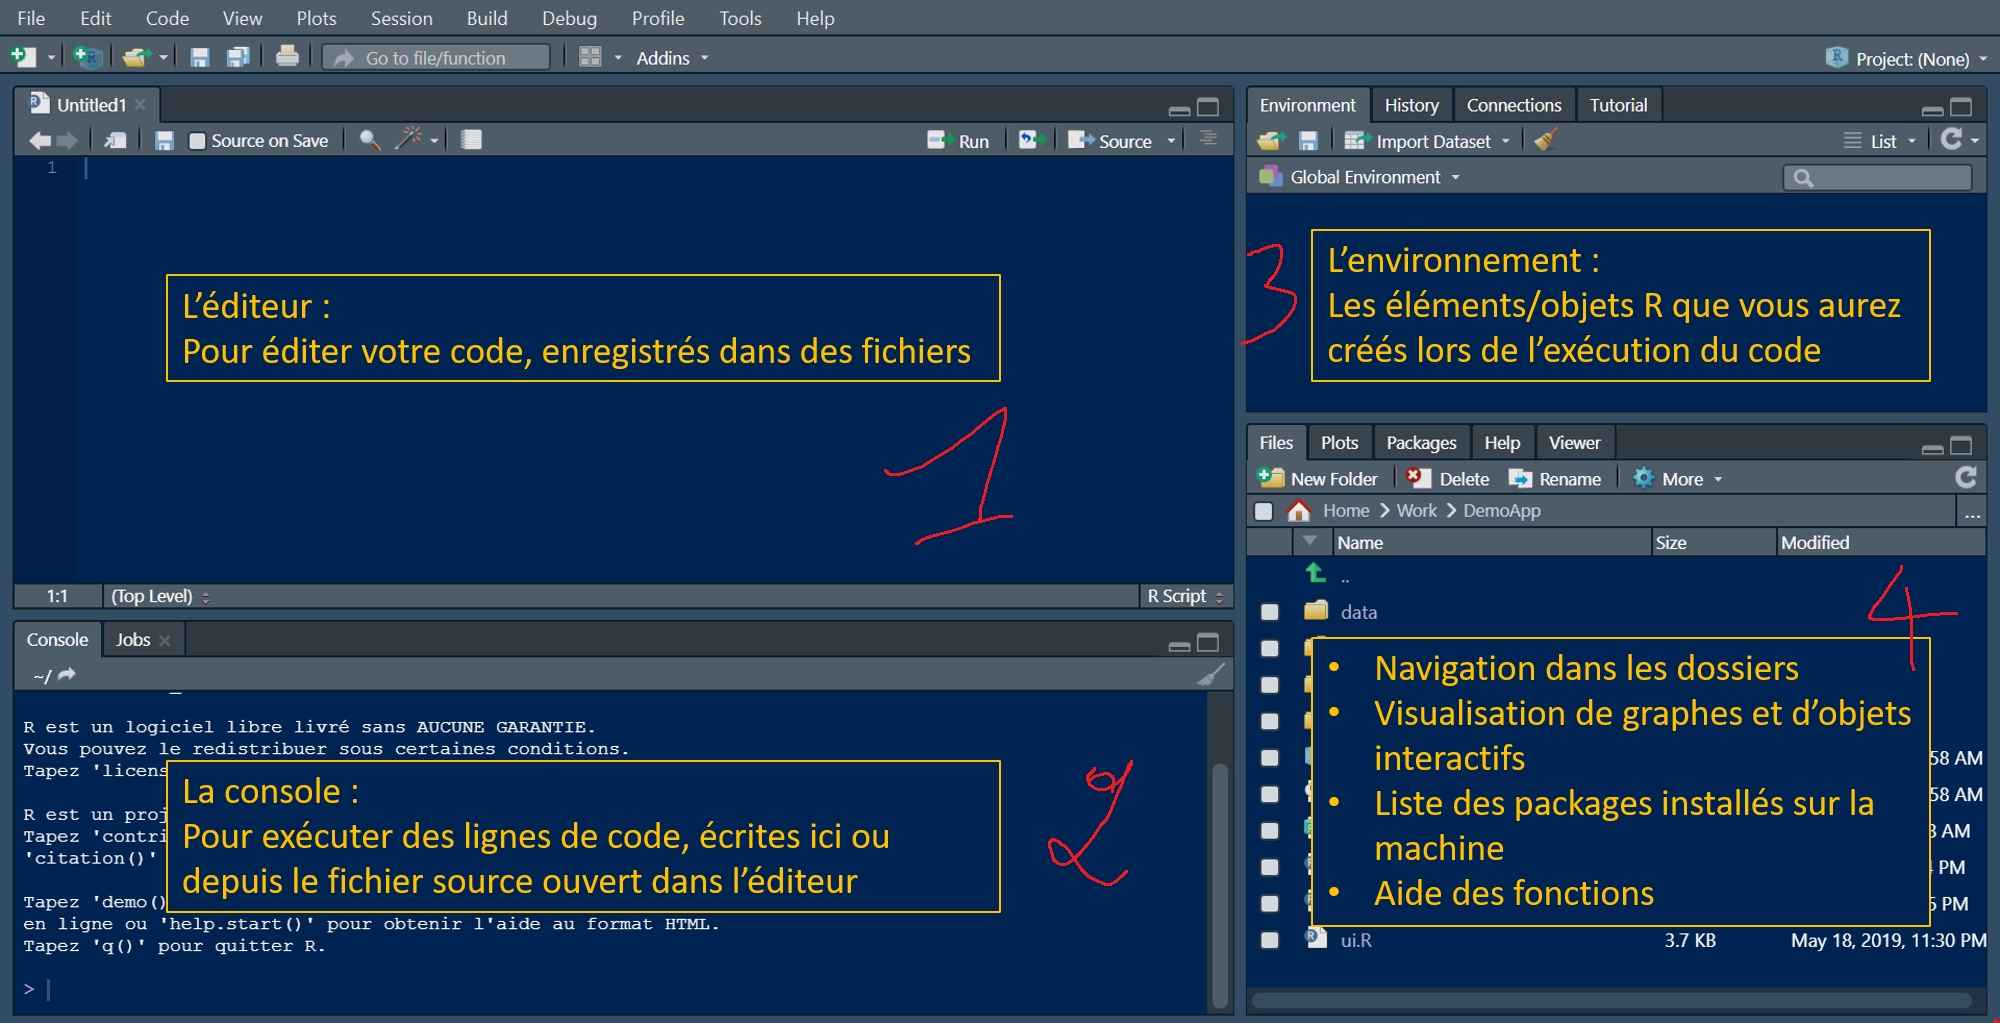
\includegraphics{interface Rstudio.png}
\caption{interface de Rstudio}
\end{figure}

\end{document}
